\expandafter\ifx\csname ifdraft\endcsname\relax
 \begin{document}
\fi

\section{結果}

以下に実験結果のグラフを示す.凡例は各グラフの下部に示した.

\subsection{低強度プロトコルと高強度プロトコルにおけるVO2}

\begin{figure}[H]
  \begin{center}
    \label{fig:light_hard_vo2}
    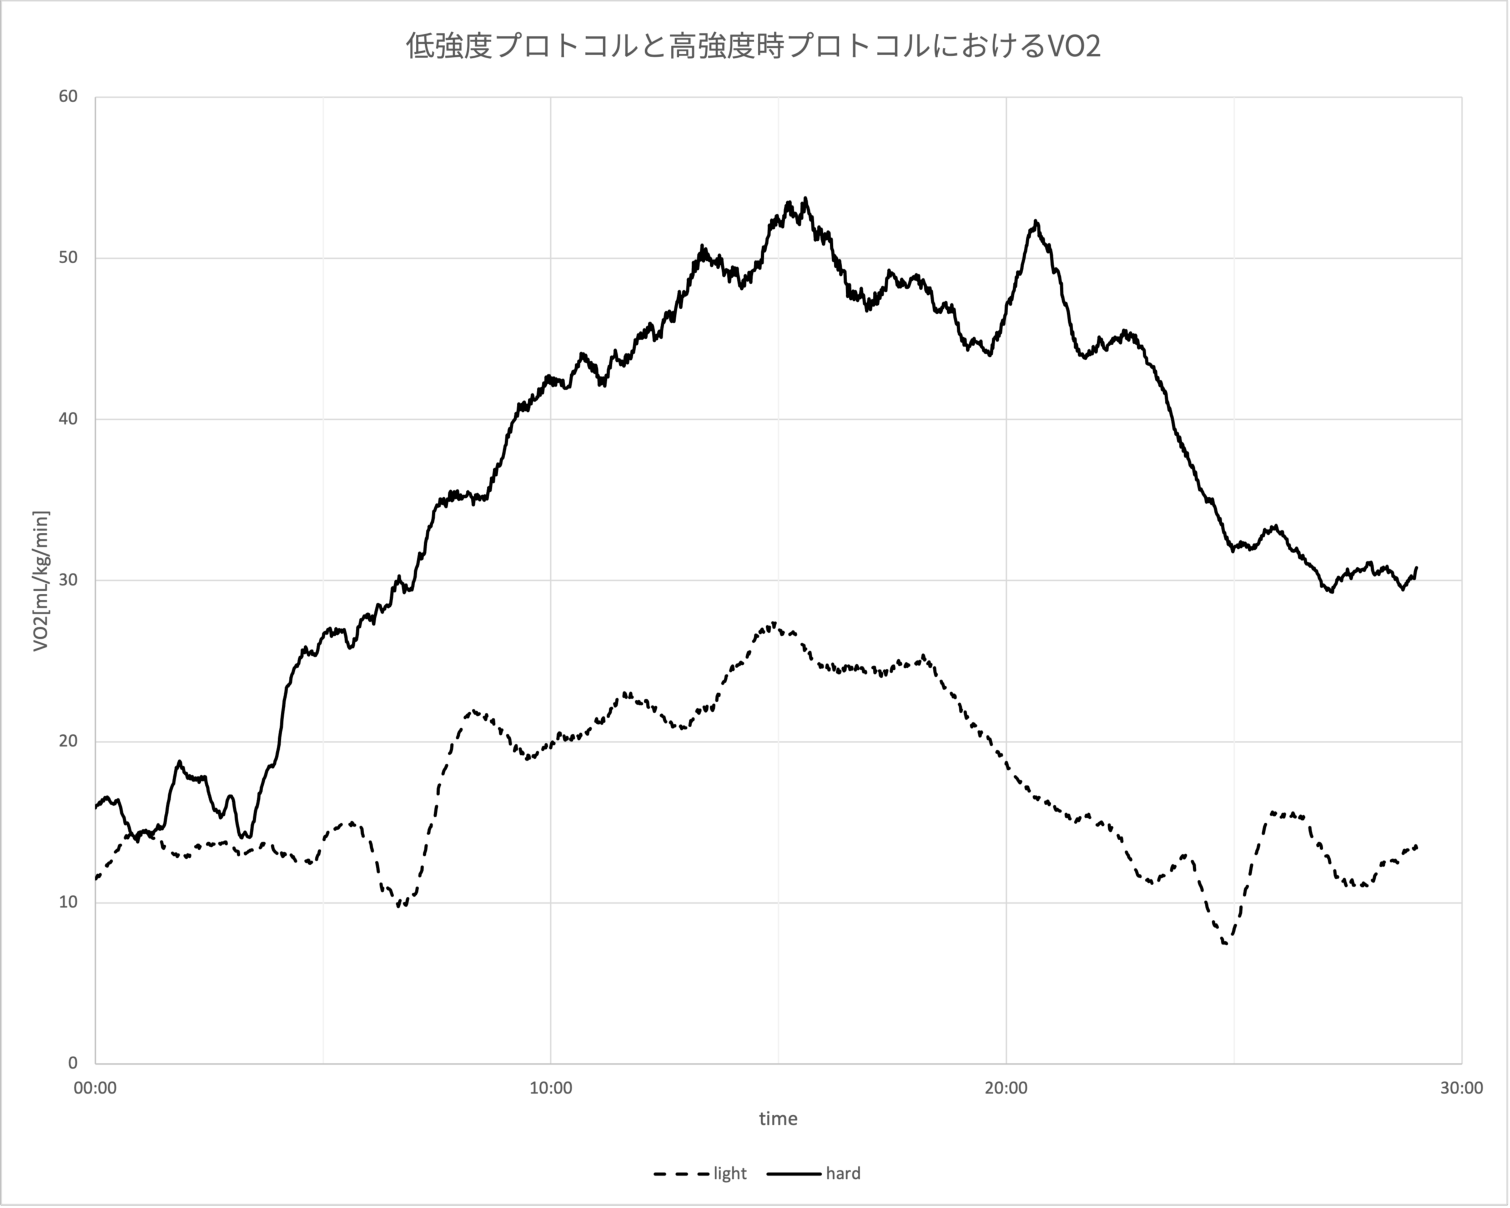
\includegraphics[width=12cm]{fig/light_hard_vo2}
    \caption{低強度プロトコルと高強度プロトコルにおけるVO2}
  \end{center}
\end{figure}

\subsection{低強度プロトコルにおけるVO2とパワー}

\begin{figure}[H]
  \begin{center}
    \label{fig:light_vo2_power}
    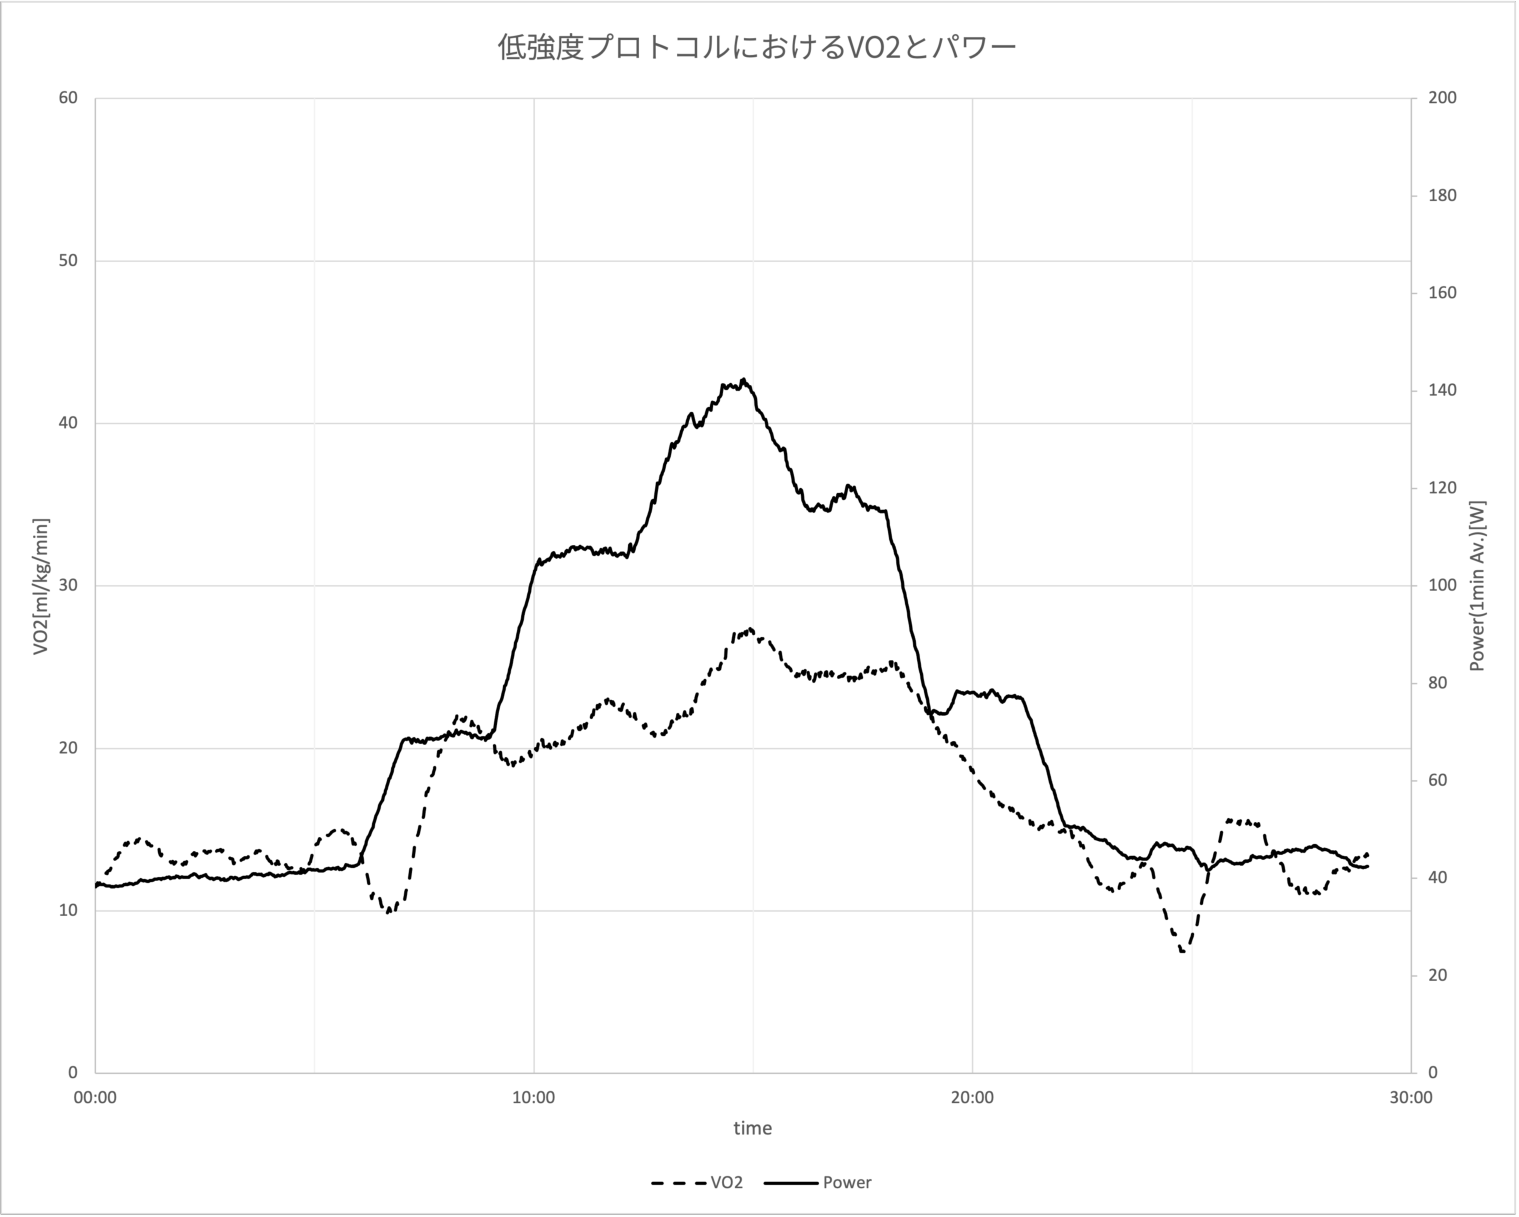
\includegraphics[width=12cm]{fig/light_vo2_power}
    \caption{低強度プロトコルにおけるVO2とパワー}
  \end{center}
\end{figure}

\subsection{低強度プロトコルにおけるVO2と心拍数}

\begin{figure}[H]
  \begin{center}
    \label{fig:light_vo2_hr}
    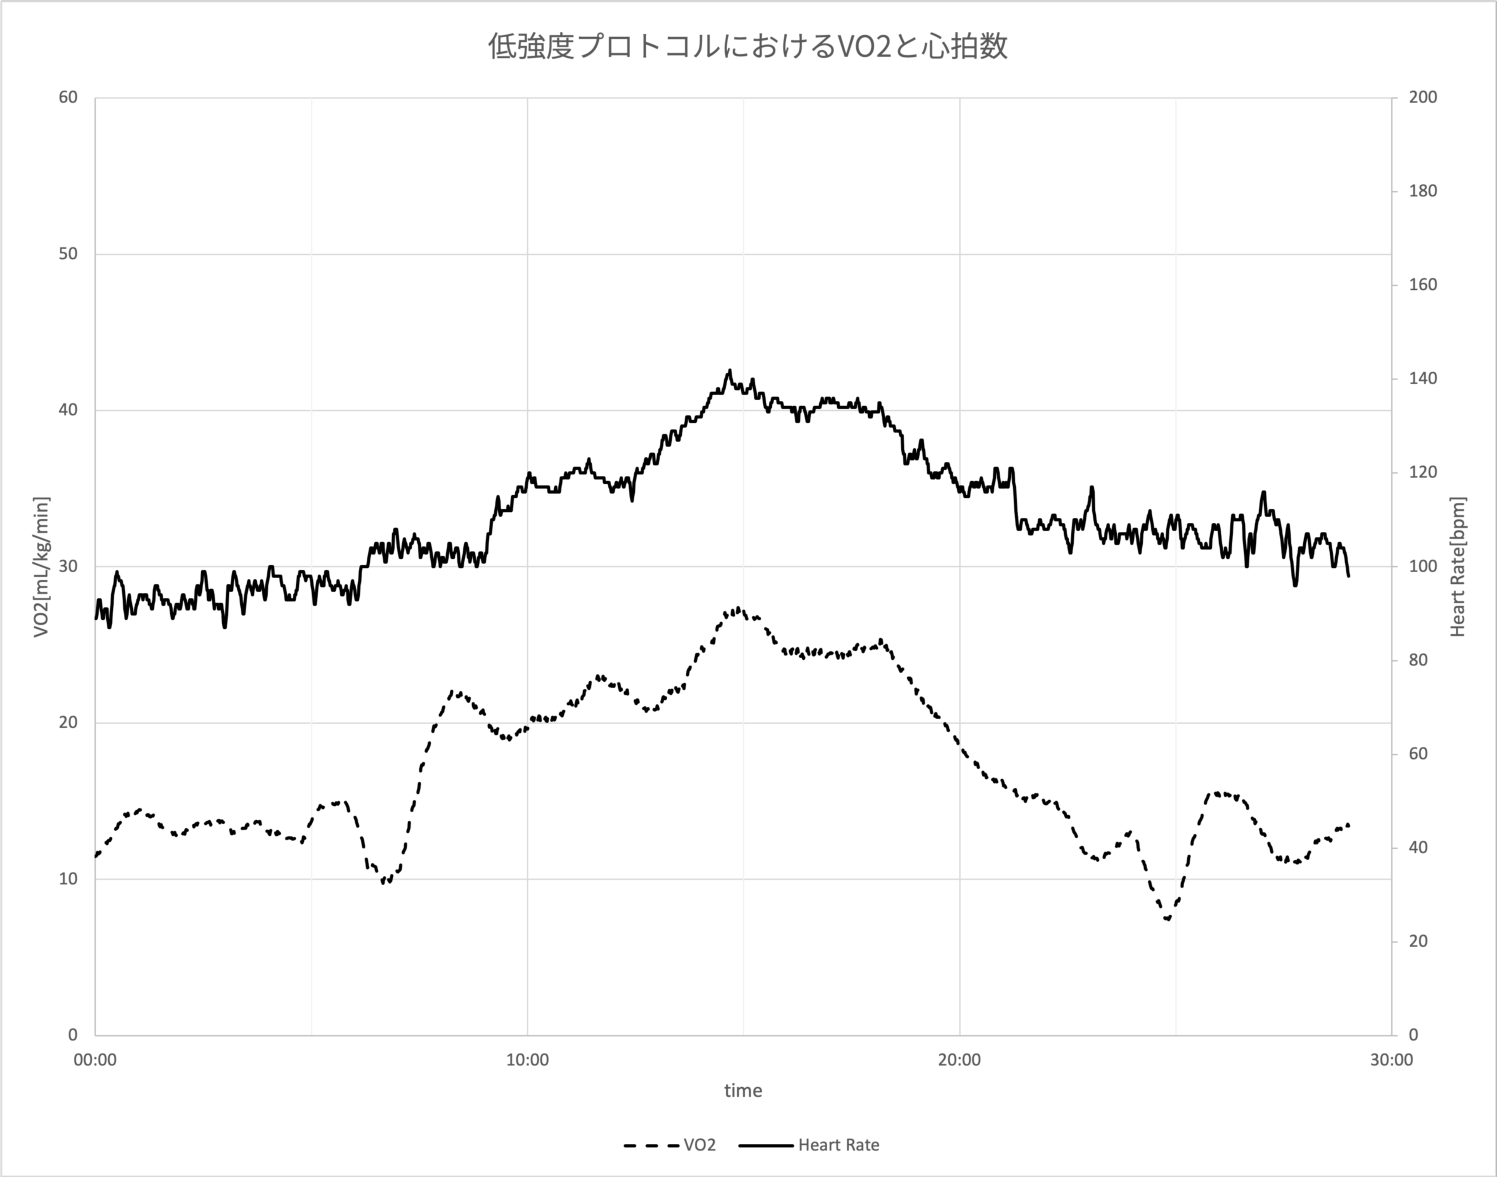
\includegraphics[width=12cm]{fig/light_vo2_hr}
    \caption{低強度プロトコルにおけるVO2と心拍数}
  \end{center}
\end{figure}

\subsection{高強度プロトコルにおけるVO2とパワー}

\begin{figure}[H]
  \begin{center}
    \label{fig:hard_vo2_power}
    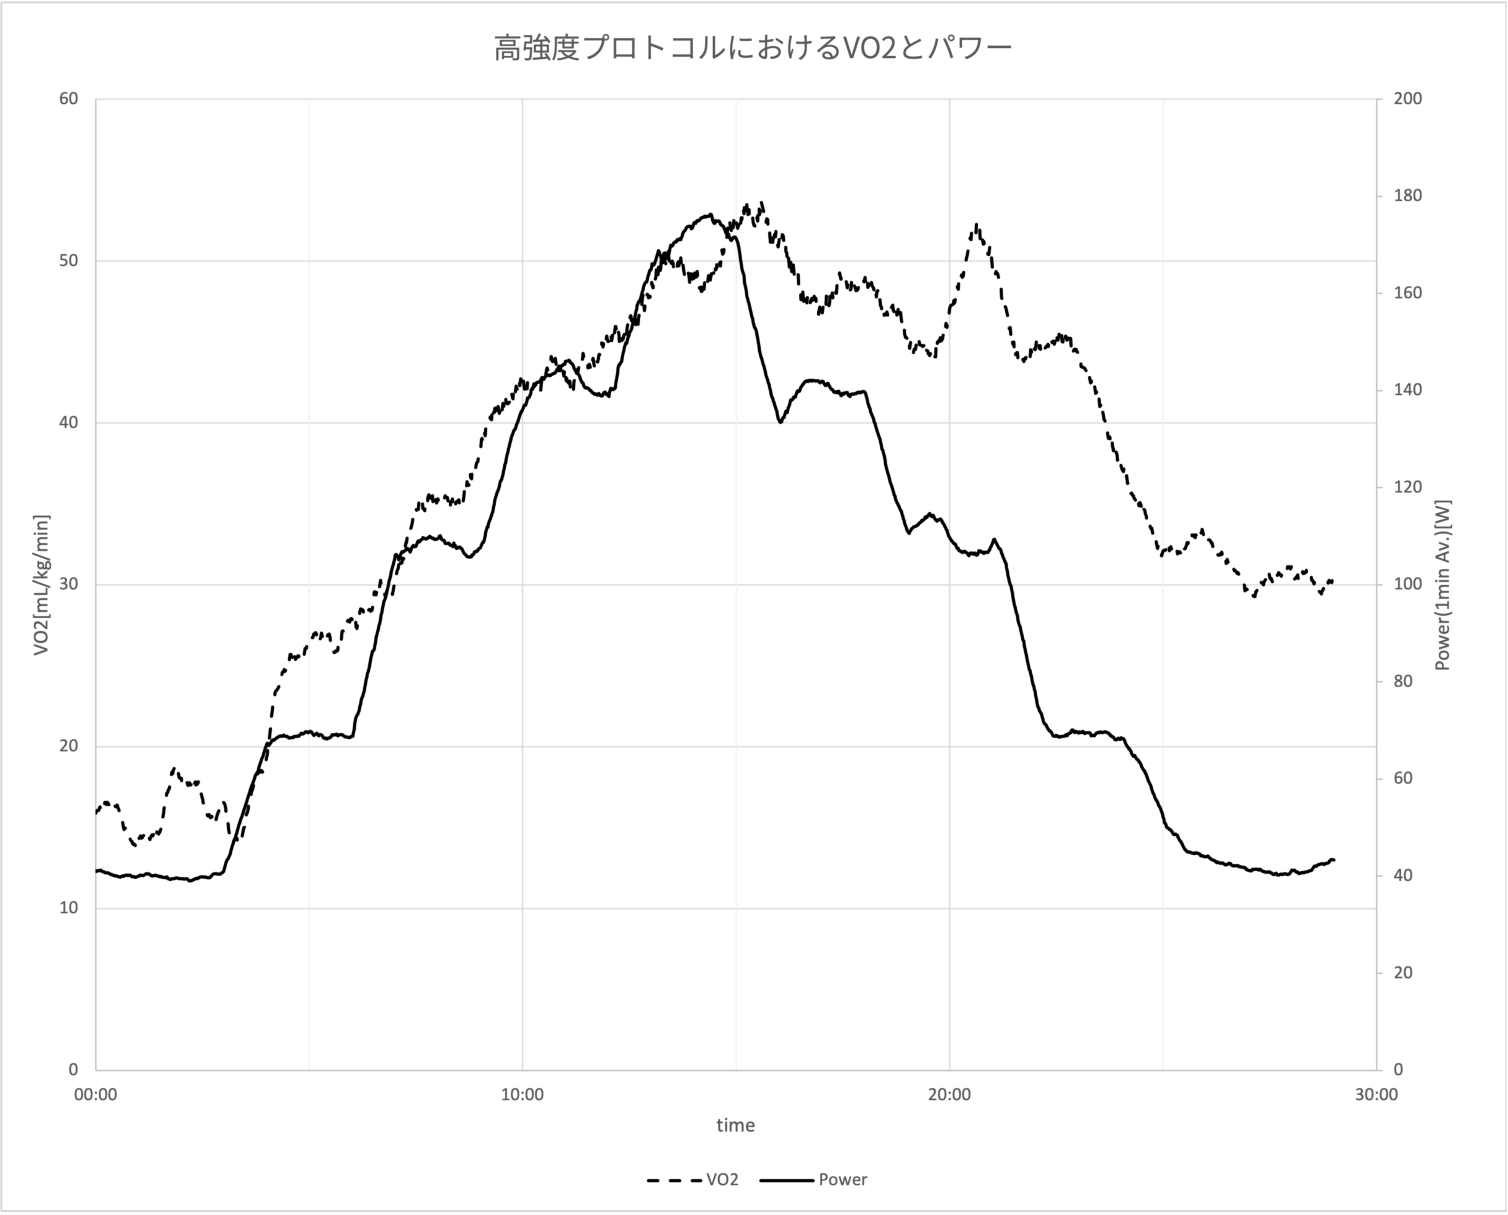
\includegraphics[width=12cm]{fig/hard_vo2_power}
    \caption{高強度プロトコルにおけるVO2とパワー}
  \end{center}
\end{figure}

\subsection{高強度プロトコルにおけるVO2と心拍数}

\begin{figure}[H]
  \begin{center}
    \label{fig:hard_vo2_hr}
    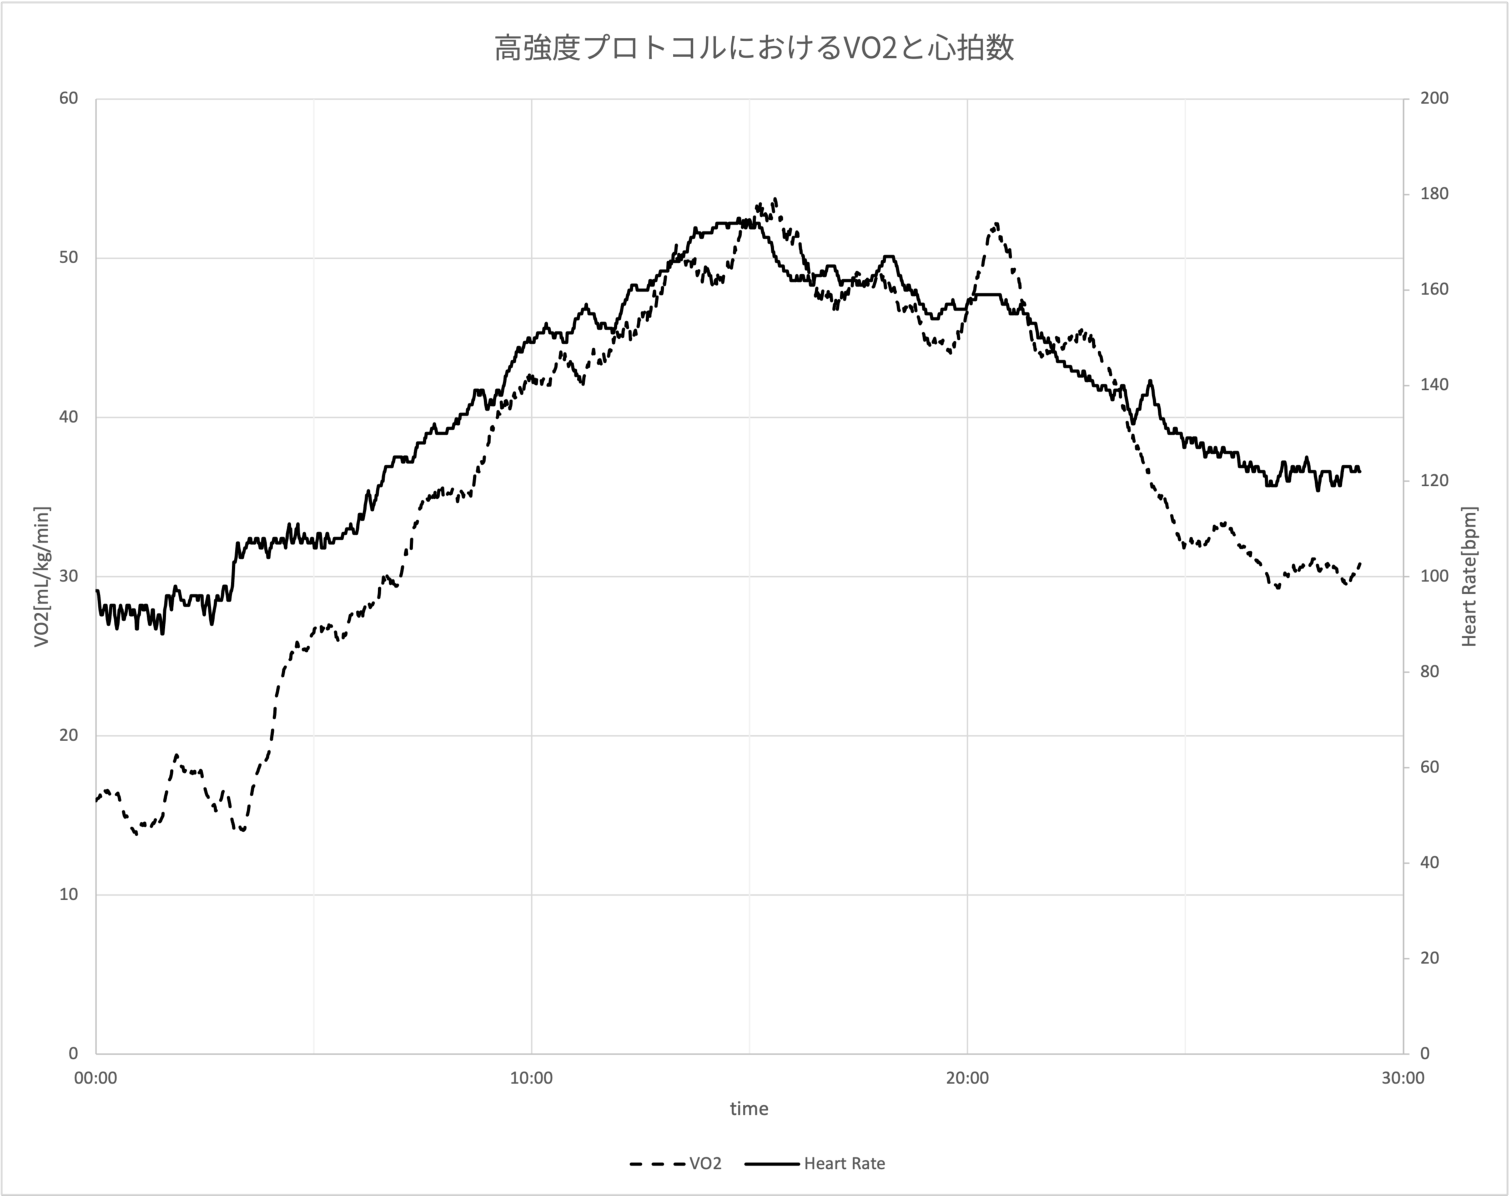
\includegraphics[width=12cm]{fig/hard_vo2_hr}
    \caption{高強度プロトコルにおけるVO2と心拍数}
  \end{center}
\end{figure}

\expandafter\ifx\csname ifdraft\endcsname\relax
  \end{document}
\fi
